\documentclass{article}
\usepackage{tikz} 
\usepackage[utf8]{inputenc}
\usepackage{amsmath}
\usepackage{listings}
\usepackage{amsfonts}
\usepackage{amssymb}
\usepackage{tabularx}
\usepackage{enumitem}
\usepackage{algorithm}% http://ctan.org/pkg/algorithm
\usepackage[noend]{algpseudocode}% http://ctan.org/pkg/algorithmicx

\usepackage{tikz}

\usepackage{graphicx}
\usetikzlibrary{arrows,positioning} 
\usepackage{subcaption}
\thispagestyle{empty}
\usepackage{multicol,caption}
\pgfarrowsdeclarecombine{ring}{ring}{}{}{o}{o}

\DeclareMathOperator{\ringarrow}{\raisebox{0.5ex}{\tikz[baseline]{\draw[ring->](0,0)--(2em,0);}}}

\tikzset{
    %Define standard arrow tip
    >=stealth',
    %Define style for boxes
    observed/.style={
           rectangle,
           rounded corners,
           draw=black, thick,
           minimum width=4em,
           minimum height=1.5em,
           font=\footnotesize,
           text centered,
           fill=blue!20!white},
     latent/.style={
           circle,
           rounded corners,
           draw=black, thick, dashed,
           minimum width=.5em,
           minimum height=.5em,
           font=\footnotesize,
           text centered,
           fill=black!10!white
           },
    % Define arrow style
    pil/.style={
           o->,
           thick,
           shorten <=2pt,
           shorten >=2pt,},
    sh/.style={ shade, shading=axis, left color=red, right color=green,
    shading angle=45 }
    
}
   
\begin{document}
\def\ci{\perp\!\!\!\perp} % from Wikipedia

\begin{figure}
\centering
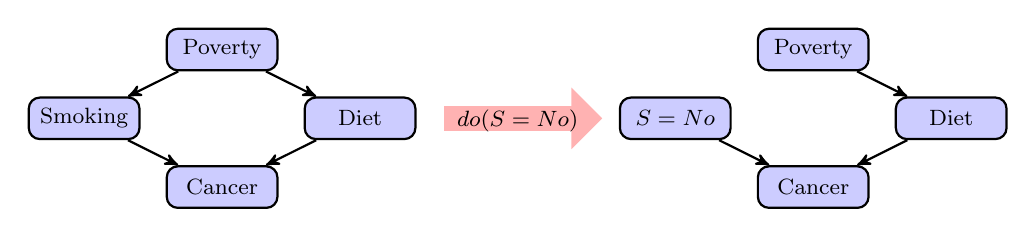
\begin{tikzpicture}[->,shorten >=0pt,shorten <=0pt,node distance=0.45cm,  thick,obs/.style={observed}, shaded/.style={latent}]
\node[obs](1){Poverty};
\node[obs,below left=of 1](2){Smoking};
\node[obs,below right=of 1](3){Diet};
\node[obs, below right = of 2](4){Cancer};
\path[] (1) edge (2) 
			edge (3) 
		(2) edge (4)
		(3) edge (4);
		
\node[obs, right = of 1, xshift=16em](5){Poverty};
\node[obs,below left=of 5](6){$S=No$};
\node[obs,below right=of 5](7){Diet};
\node[obs, below right = of 6](8){Cancer};
\path[every node/.style={font=\sffamily\footnotesize}]
(3) edge [-, >=stealth', red!30!white, line width=.9em,shorten <=1em,shorten >= 1.7em,
	preaction={line width = .3em, red!30!white,-triangle 90,draw,shorten >=.6em,shorten <=1em}] node[black,yshift=-.09em]{$do(S=No)$} (6) 
		(5) edge (7)  
		(6) edge (8)
		(7) edge (8);
		
\end{tikzpicture}

\end{figure}

\end{document}